\section{Shadertoy}

\begin{frame}{Una idea ingeniosa}
Todo empezó con una \href{https://iquilezles.org/articles/nvscene2008/rwwtt.pdf}{plática}: \say{Rendering Worlds With Two Triangles} presentada en la \href{https://www.youtube.com/watch?v=A1iW6Z_Jc4k}{conferencia NVScene} el 22 Aug 2008 por \href{https://iquilezles.org/}{Iñigo Quilez}.
\begin{exampleblock}{}
\begin{enumerate}
    \item Si dibujamos un cuadrado (formado por 2 triángulos), que cubre toda la ventana. Esto provocará la ejecución del fragment (pixel) shader en todos los píxeles de la pantalla. 
    \item Luego, usamos el fragment shader en donde cada fragment (pixel) sabe su respectiva posición en el render target, unas constantes (uniforms) y un montón de matemáticas, para dibujar la escena.
\end{enumerate}
\end{exampleblock}
\begin{figure}[htp]
  \centering
  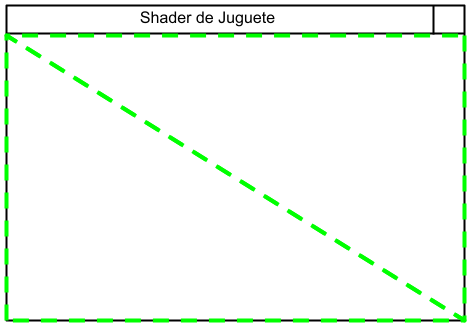
\includegraphics[width=0.2\textwidth]{img/TwoTriangles}
\end{figure}
\end{frame}

\begin{frame}{Regresar al principio}
\begin{figure}[htp]
  \centering
  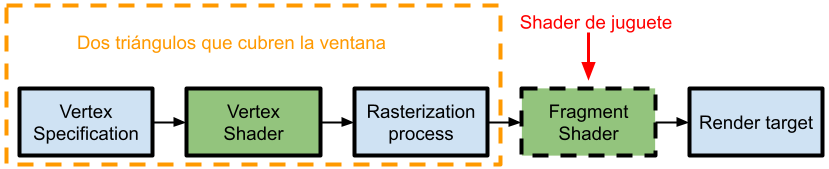
\includegraphics[width=0.7\textwidth]{img/Truco}
\end{figure}
\begin{itemize}
    \item Es similar a como se hacían los gráficos antes de que tuviéramos tarjetas de video.
    \item Solo que ahora aprovechamos el \alert{inmenso poder paralelo} del GPU.
    \item Y usamos GLSL.
\end{itemize}
\end{frame}

\begin{frame}{Nota curiosa}
\begin{figure}[htp]
  \centering
  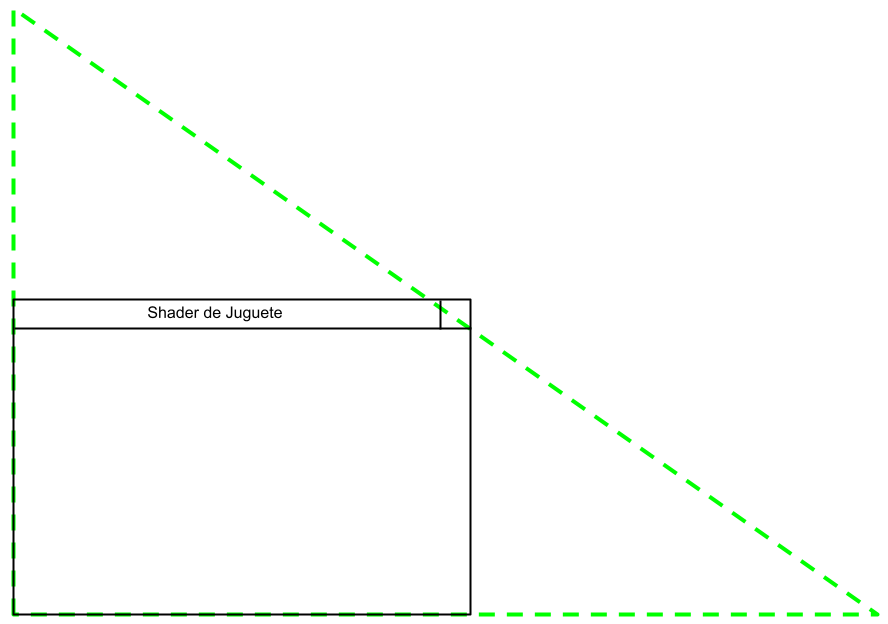
\includegraphics[width=0.4\textwidth]{img/onetriangle}
\end{figure}
De hecho podemos hacerlo con un solo triángulo y luego hacemos clipping.
\end{frame}

\begin{frame}{Actualmente, es mejor hacer:}
\begin{figure}[htp]
  \centering
  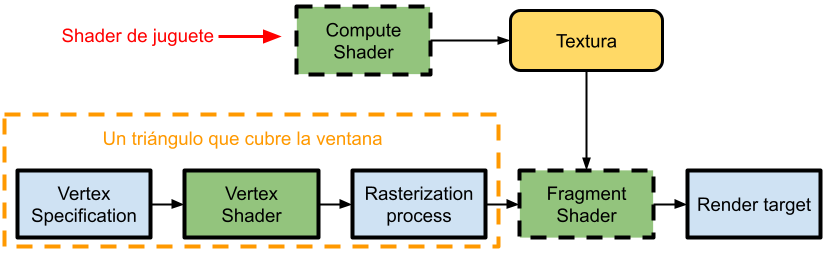
\includegraphics[width=0.65\textwidth]{img/TrucoModerno}
\end{figure}
\end{frame}

\begin{frame}{Shadertoy}
\begin{itemize}
    \item Shadertoy es un sitio web: \url{https://www.shadertoy.com/} que nos da la infraestructura para usar el truco.
    \item Y ciertas herramientas sociales.
    \item Fue creado por \href{https://iquilezles.org/}{Iñigo Quilez} y \href{https://www.poljeremias.com/}{Pol Jeremias} en el 2013.
\end{itemize}
\begin{figure}[htp]
  \centering
  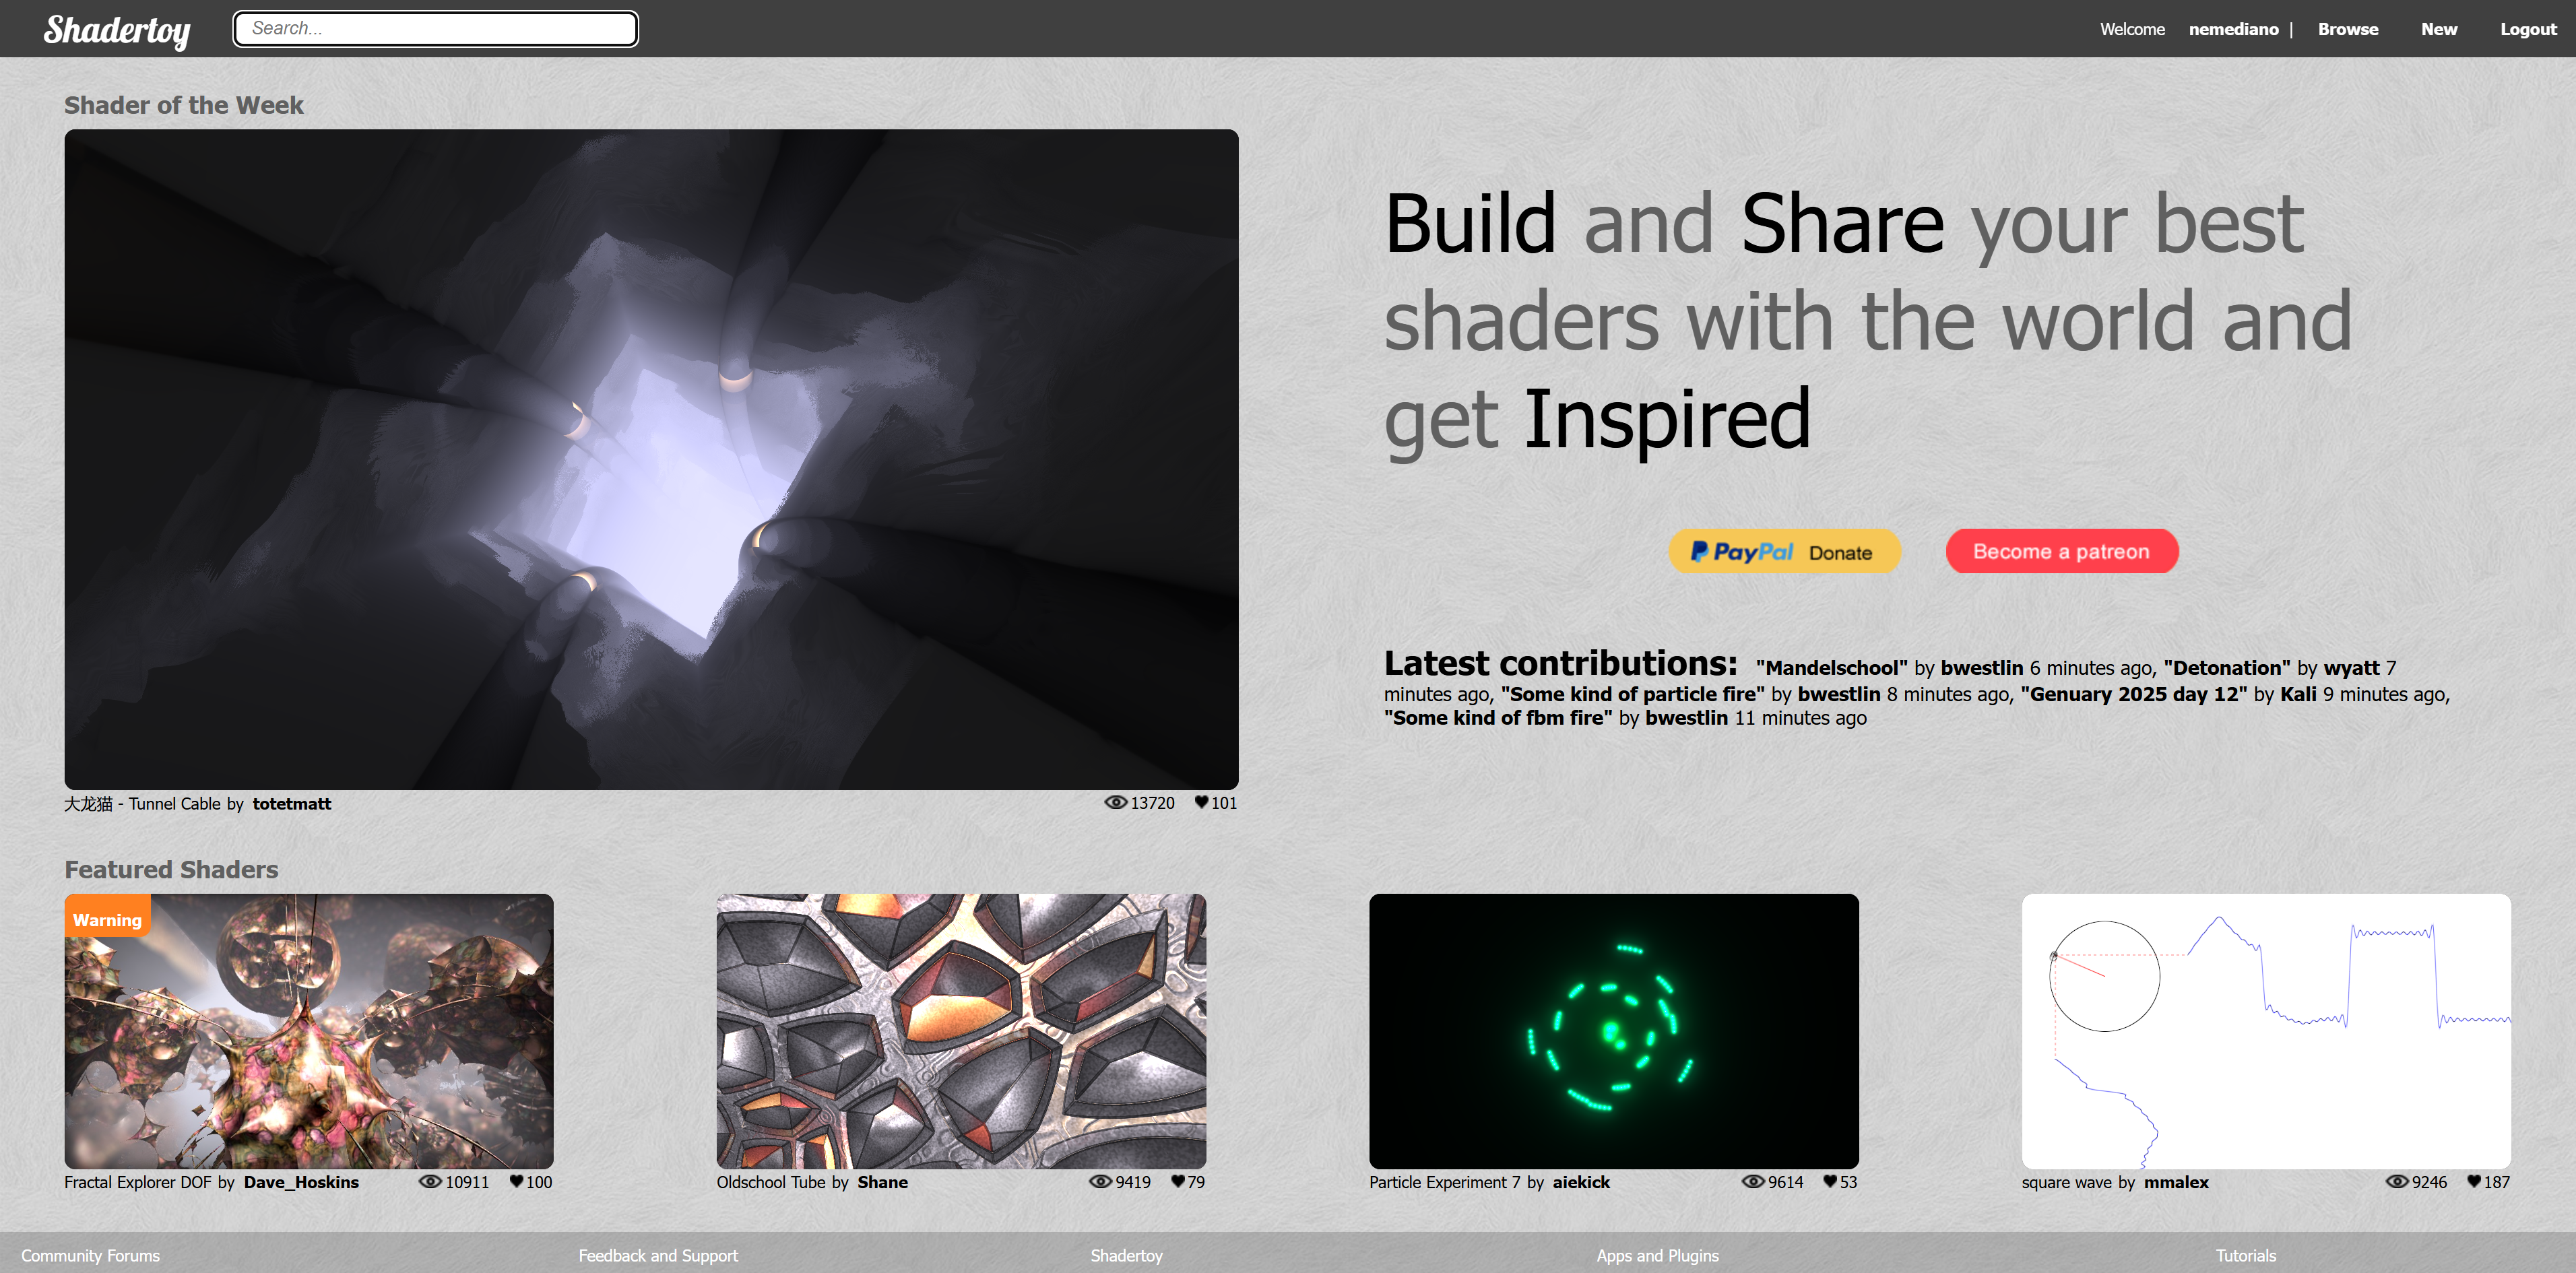
\includegraphics[width=0.4\textwidth]{img/ShaderToySite}
\end{figure}
\end{frame}

\begin{frame}{¿Cómo se usa?}
Escribir un programa en \href{https://www.khronos.org/opengl/wiki/Core_Language_(GLSL)}{GLSL} que se ejecuta en paralelo por cada pixel de la salida.
\begin{itemize}
    \item \textbf{Entradas:} recibes la coordenada del pixel.
    \item \textbf{Salida:} debes regresar el color del pixel.
    \item Recibe algunas constantes extra: el tiempo, el tamaño total del render target, etc.
\end{itemize}
\begin{figure}[htp]
  \centering
  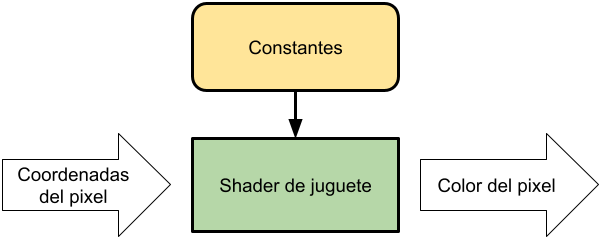
\includegraphics[width=0.4\textwidth]{img/SimpleShaderToy}
\end{figure}
\end{frame}

\begin{frame}{Así se ve}
\begin{figure}[htp]
  \centering
  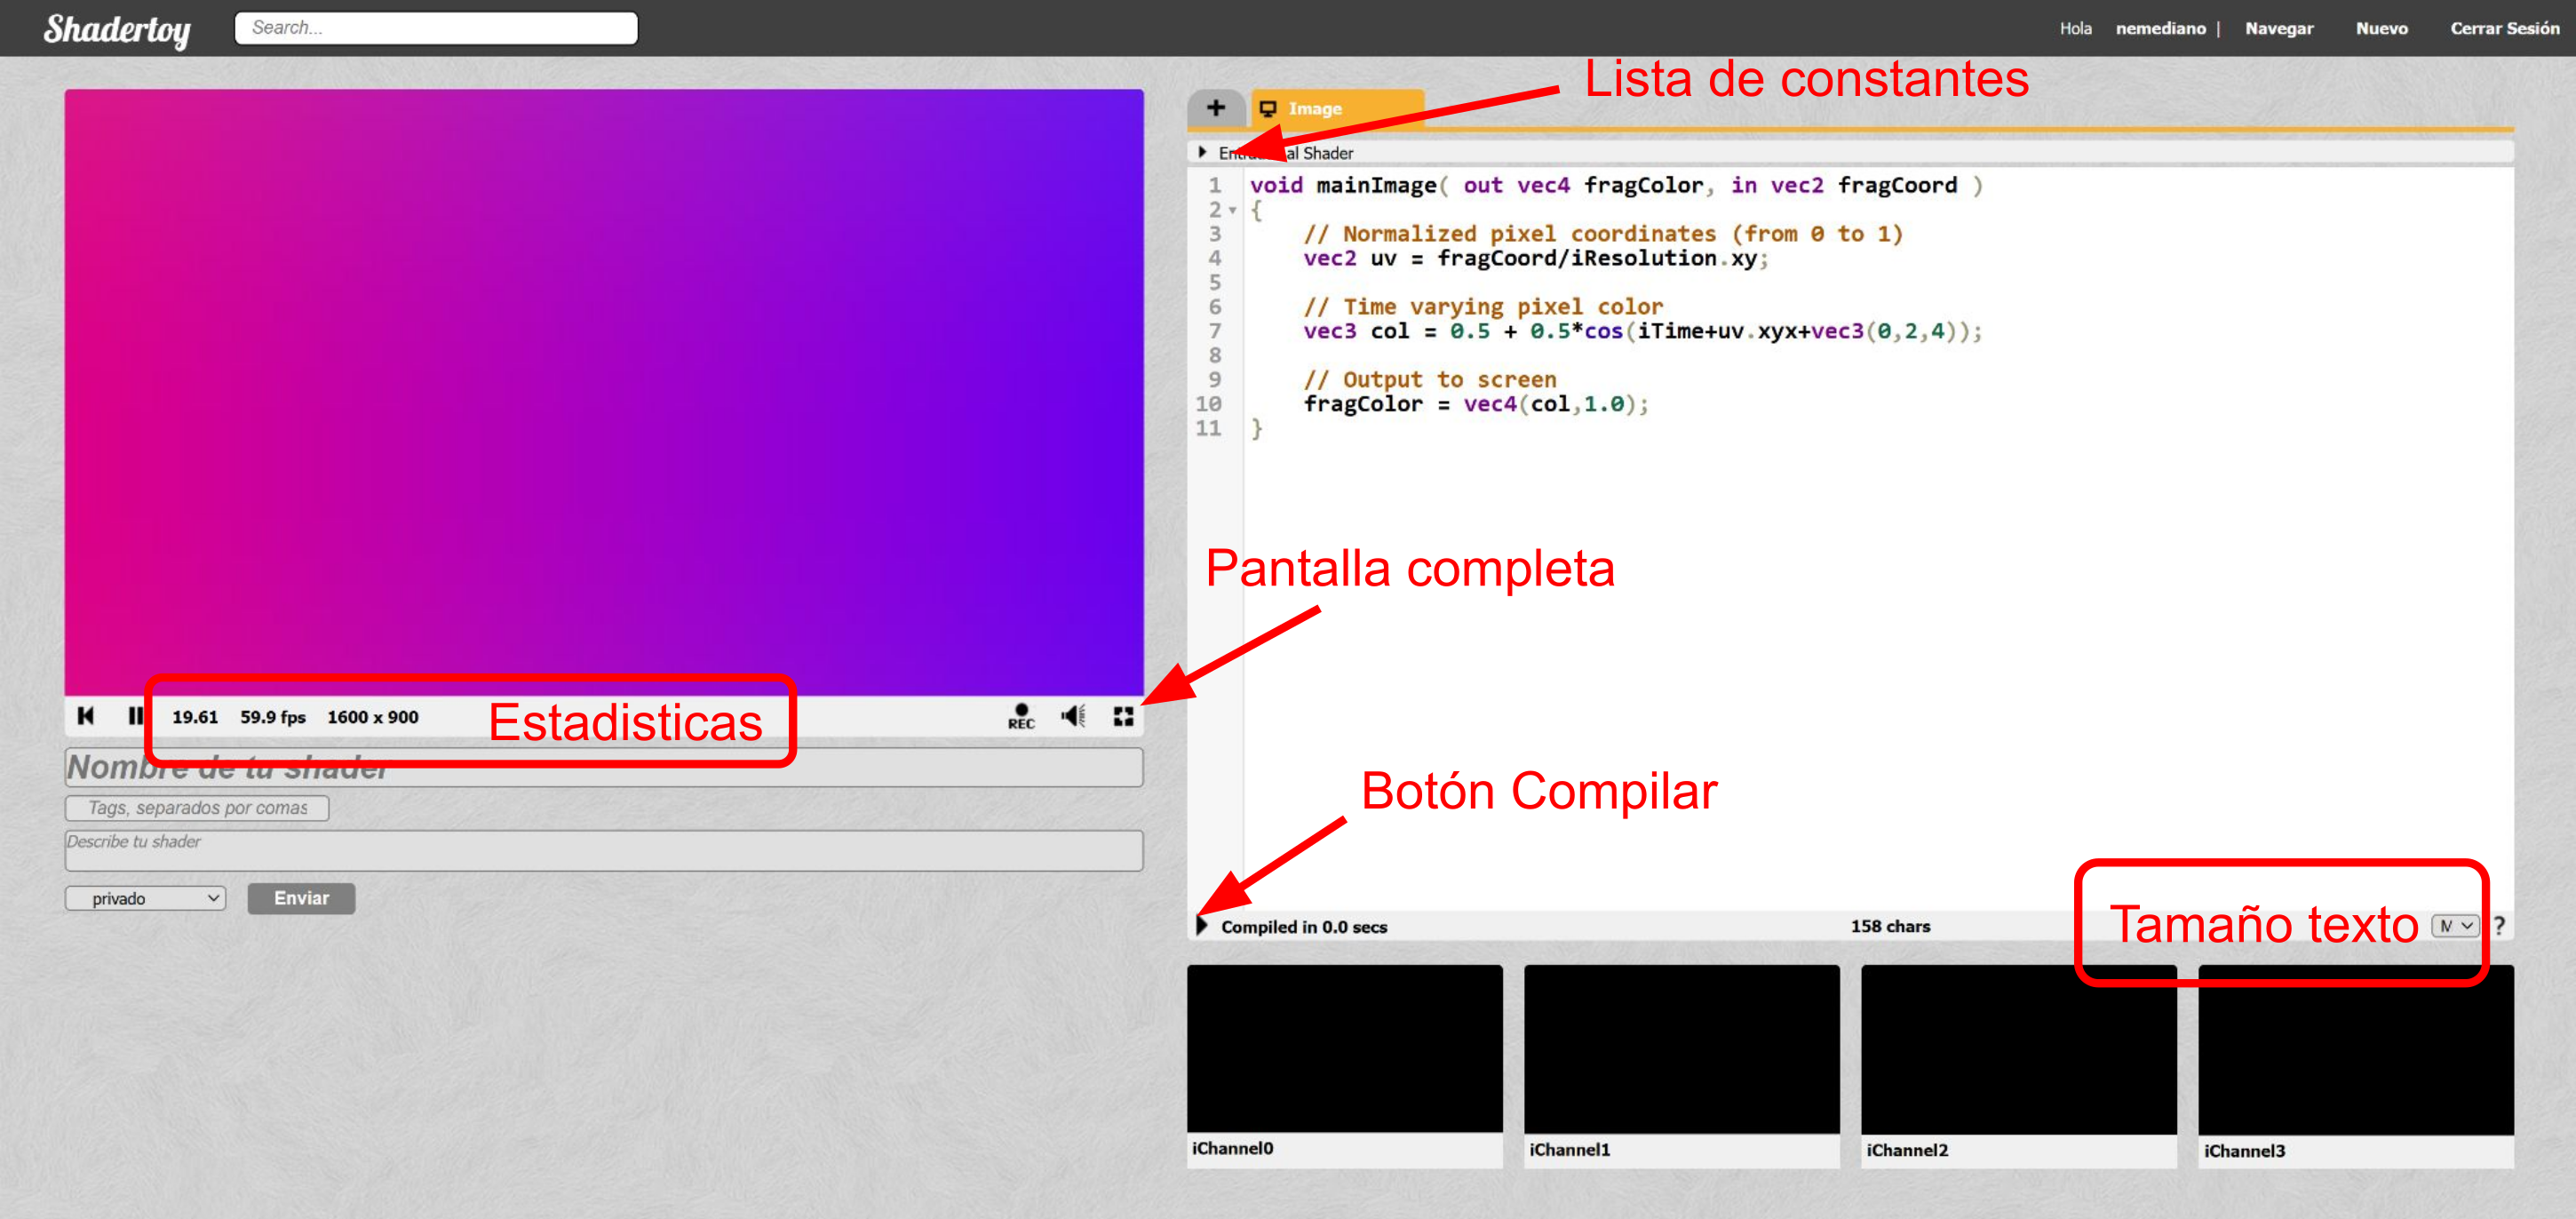
\includegraphics[width=0.8\textwidth]{img/ShaderToyUI}
\end{figure}
\end{frame}

\begin{frame}{Portabilidad}
Shadertoy:
\begin{itemize}
    \item Crea el pipeline por nosotros.
    \item Inyecta código en el fragment shader.
\end{itemize}
Pero ten por seguro que:
\begin{block}{}
    Cualquier shader que funciona en shadertoy, puede ser \alert{portado} y funcionar en cualquier otro entorno que pueda desplegar gráficos.
\end{block}
Adicionalmente:
\begin{itemize}{}
    \item Hay muchos entornos de programación, que emulan Shadertoy.
    \item Siempre puedes escribir tu propio programa que ejecute shaders de shadertoy.
\end{itemize}
\begin{block}{}
    No es tan difícil, cualquier alumno que haya tomado una clase de CG puede hacerlo fácilmente.
\end{block}
\end{frame}
